\documentclass[final]{beamer}
%% Possible paper sizes: a0, a0b, a1, a2, a3, a4.
%% Possible orientations: portrait, landscape
%% Font sizes can be changed using the scale option.
\usepackage[size=a1,orientation=portrait,scale=1.1]{beamerposter}

\usetheme{gemini}
\usecolortheme{seagull}
\useinnertheme{rectangles}

% ====================
% Packages
% ====================

\usepackage[utf8]{inputenc}
\usepackage{graphicx}
\usepackage{booktabs}
\usepackage{tikz}
\usepackage{pgfplots}
\usepackage{svg}
\usepackage{amsmath,amssymb,amsfonts}
\usepackage{multicol}
\usepackage{placeins}
\usepackage[noend]{algpseudocode}
\usepackage{amsmath}
 

% ====================
% Lengths
% ====================

% If you have N columns, choose \sepwidth and \colwidth such that
% (N+1)*\sepwidth + N*\colwidth = \paperwidth
\newlength{\sepwidth}
\newlength{\colwidth}
\setlength{\sepwidth}{0.03\paperwidth}
\setlength{\colwidth}{0.45\paperwidth}

\newcommand{\separatorcolumn}{\begin{column}{\sepwidth}\end{column}}

% ====================
% Logo (optional)
% ====================

% LaTeX logo taken from https://commons.wikimedia.org/wiki/File:LaTeX_logo.svg
% use this to include logos on the left and/or right side of the header:
\logoleft{
\includegraphics[height=6.6cm]{logo/iub_cse.png}}
\logoright{
\includegraphics[height=6.6cm]{logo/iub_logo.png}}

% ====================
% Footer (optional)
% ====================

\footercontent{
	\insertdate \hfill
	Algorithm Project \hfill
	CSE211: Algorithms Lab
    % \href{mailto:myemail@exampl.com}{\texttt{myemail@example.com}}
}
% (can be left out to remove footer)

% ====================
% My own customization
% - BibLaTeX
% - Boxes with tcolorbox
% - User-defined commands
% ====================
% ====================
% BibLaTeX
% ====================

\usepackage[backend=biber,
	bibstyle=authoryear,
	citestyle=authoryear,
	style=authoryear,
	maxcitenames=2,
	maxbibnames=20, % limit the length of list of names (authors/editors/etc.)
	sorting=ydnt, % sort references by year (descending), name, title
	dashed=false, % show authors instead of dash in publications having the same authors
	giveninits=true % render authors' given name initials and not the full given names
]{biblatex}
%% Biblatex with Beamer bibliography icons
\setbeamertemplate{bibliography item}{%
	\ifboolexpr{ test {\ifentrytype{book}} or test {\ifentrytype{mvbook}}
		or test {\ifentrytype{collection}} or test {\ifentrytype{mvcollection}}
		or test {\ifentrytype{reference}} or test {\ifentrytype{mvreference}} }
	{\setbeamertemplate{bibliography item}[book]}
	{\ifentrytype{online}
		{\setbeamertemplate{bibliography item}[online]}
		{\setbeamertemplate{bibliography item}[article]}}%
	\usebeamertemplate{bibliography item}}
\defbibenvironment{bibliography}
{\list{}
	{\settowidth{\labelwidth}{\usebeamertemplate{bibliography item}}%
		\setlength{\leftmargin}{\labelwidth}%
		\setlength{\labelsep}{\biblabelsep}%
		\addtolength{\leftmargin}{\labelsep}%
		\setlength{\itemsep}{\bibitemsep}%
		\setlength{\parsep}{\bibparsep}}}
{\endlist}
{\item}
%% Redefine \refname
\renewcommand{\bibname}{References}
%% Redefine \parencite to use square brackets instead of braces
\DeclareCiteCommand{\parencite}
{\usebibmacro{prenote}}
{\usebibmacro{citeindex}%
	\printtext[bibhyperref]{[\usebibmacro{cite}]}}
{\multicitedelim}
{\usebibmacro{postnote}}
%% Highlight author names using Beamer data annotation
%% Usage: add a new line `author+an = {<author-order>=highlight}` to an entry
%% For example: author+an = {3=highlight} => highlight the 3rd author name
\AtBeginBibliography{
	\renewcommand*{\mkbibnamegiven}[1]{%
		\ifitemannotation{highlight}
		{\textbf{#1}}
		{#1}%
	}
	
	\renewcommand*{\mkbibnamefamily}[1]{%
		\ifitemannotation{highlight}
		{\textbf{#1}}
		{#1}%
	}
}

% ====================
% Boxes with tcolorbox
% ====================
\usepackage[most]{tcolorbox}

%%% Beamer colors in boxes

\newcommand{\beamercolorsinboxes}[1]{
	\setbeamercolor{itemize item}{fg=#1!75!black}
	\setbeamercolor{itemize/enumerate body}{fg=#1!65!white}
	\setbeamercolor{itemize/enumerate subbody}{fg=#1!65!white}
	\setbeamercolor{item projected}{fg=white, bg=#1!75!black}
}

%%% Highlight Oval Box
\newtcbox{\xmybox}[1][red]{on line,
	arc=7pt,colback=#1!10!white,colframe=#1!50!black,
	before upper={\rule[-3pt]{0pt}{10pt}},boxrule=1pt,
	boxsep=0pt,left=6pt,right=6pt,top=2pt,bottom=2pt}
%%% Box for stating problems
%%%%%%%%
%Usage: (similar for infobox)
%	\begin{defbox}{title}
	%		contents
	%	\end{defbox}
%%%%%%%%
\newtcolorbox{defbox}[1]{%
	enhanced,
	attach boxed title to top 	left={xshift=5mm,yshift=-5mm,yshifttext=-5mm},
	colback=cyan!5!white,
	colframe=cyan!75!black,
	coltitle=cyan!80!black,
%	left=0mm,right=0mm,top=2mm,bottom=0mm,
	title={#1},
	fonttitle=\bfseries\large, fontupper=\color{cyan!65!white},
	boxed title style={colback=cyan!5!white,colframe=cyan!75!black},
	before upper={
		\beamercolorsinboxes{cyan}
	}
}%
%%% Box for announcement
\newtcolorbox{infobox}[1]{%
	enhanced,
	attach boxed title to top 	left={xshift=5mm,yshift=-5mm,yshifttext=-5mm},
	colback=yellow,
	colframe=red!75!black,
	coltitle=red!75!black,
%	left=0mm,right=0mm,top=2mm,bottom=0mm,
	title={#1},
	fonttitle=\bfseries\large, fontupper=\color{red!65!white},
	boxed title style={colback=yellow,colframe=red!75!black},
	before upper={
		\beamercolorsinboxes{red}
	}
}%
%%% Box for example
\newtcolorbox{exabox}[1]{%
	enhanced,
	attach boxed title to top 	left={xshift=5mm,yshift=-5mm,yshifttext=-5mm},
	colframe=brown!75!black,colback=brown!5!white,coltitle=brown!50!brown!75!black,
%	left=0mm,right=0mm,top=2mm,bottom=0mm,
	title={#1},
	fonttitle=\bfseries\large, fontupper=\color{brown!65!white},
	boxed title style={colback=brown!5!white,coltitle=brown!50!brown!75!black},
	before upper={
		\beamercolorsinboxes{brown}
	}
}%
%%% Theorem Box
%%%%%%%%
%Usage: (similar for conjecture, lemma, etc.)
%	\begin{thm}{title}{nameref}
	%		contents
	%	\end{thm}
% Use \ref{thm:nameref} to refer to the theorem
%%%%%%%%
%%%% Use \newtcbtheorem[number within=section]{thm} to number within each section
\newtcbtheorem[]{thm}%
{Theorem}{attach boxed title to top 	left={xshift=5mm,yshift=-5mm,yshifttext=-5mm},
	enhanced jigsaw,
	%	top=2mm,bottom=0mm,left=0mm,right=0mm,
	fonttitle=\bfseries\large,fontupper=\itshape\color{blue!65!white},
	colframe=blue!75!black,colback=blue!5!white,coltitle=blue!50!blue!75!black,
	boxed title style={colback=blue!5!white,coltitle=blue!50!blue!75!black},
	before upper={
		\beamercolorsinboxes{blue}
	}
}{thm}%
%%% Proposition Box
\newtcbtheorem[use counter from=thm]{prop}%
{Proposition}{attach boxed title to top 	left={xshift=5mm,yshift=-5mm,yshifttext=-5mm},
	enhanced jigsaw,
	%	top=2mm,bottom=0mm,left=0mm,right=0mm,
	fonttitle=\bfseries\large,fontupper=\itshape,
	colframe=gray!75!black,colback=gray!5!white,coltitle=gray!50!gray!75!black,
	boxed title style={colback=gray!5!white,coltitle=gray!50!gray!75!black},
	before upper={
		\beamercolorsinboxes{gray}
	}
}{prop}%
%%% Conjecture Box
\newtcbtheorem[use counter from=thm]{conj}%
{Conjecture}{attach boxed title to top 	left={xshift=5mm,yshift=-5mm,yshifttext=-5mm},
	enhanced jigsaw,
	%	top=2mm,bottom=0mm,left=0mm,right=0mm,
	fonttitle=\bfseries\large,fontupper=\slshape,
	colframe=orange!75!black,colback=orange!5!white,coltitle=orange!50!orange!75!black,
	boxed title style={colback=orange!5!white,coltitle=orange!50!orange!75!black},
	before upper={
		\beamercolorsinboxes{orange}
	}
}{conj}%
%%% Lemma Box
\newtcbtheorem[use counter from=thm]{lem}%
{Lemma}{attach boxed title to top 	left={xshift=5mm,yshift=-5mm,yshifttext=-5mm},
	enhanced jigsaw,
	%	top=2mm,bottom=0mm,left=0mm,right=0mm,
	fonttitle=\bfseries\large,fontupper=\itshape,
	colframe=green!75!black,colback=green!5!white,coltitle=green!50!green!75!black,
	boxed title style={colback=green!5!white,coltitle=green!50!green!75!black},
	before upper={
		\beamercolorsinboxes{green}
	}
}{lem}%
%%% Claim Box
\newtcbtheorem[use counter from=thm]{clm}%
{Claim}{attach boxed title to top 	left={xshift=5mm,yshift=-5mm,yshifttext=-5mm},
	enhanced jigsaw,
	%	top=2mm,bottom=0mm,left=0mm,right=0mm,
	fonttitle=\bfseries\large,fontupper=\itshape,
	colframe=pink!75!black,colback=pink!5!white,coltitle=pink!50!pink!75!black,
	boxed title style={colback=pink!5!white,coltitle=pink!50!pink!75!black},
	before upper={
		\beamercolorsinboxes{pink}
	}
}{clm}%

%Configs

\def\inst#1{\unskip$^{#1}$}
\def\orcidID#1{\unskip$^{[#1]}$} % added MR 2018-03-10
\def\fnmsep{\unskip$^,$}
\def\email#1{{\tt#1}}



%% Reference Sources
\addbibresource{refs.bib}
\renewcommand{\pgfuseimage}[1]{\includegraphics[scale=2.0]{#1}}

\pgfplotsset{compat=1.18}



\title{RADIX SORT UNRAVELED}

\author
{
    Sabbir Islam \inst{1} \and
    Anika Tabassum \inst{2} \and
    Sadnan Yasar Tanvir\inst{3} \and 
    Samia Reza Maisha \inst{4} 
    Saiful Islam \inst{5}     
}

% \institute[shortinst]{\inst{1} Independent University Bangladesh \samelineand \inst{2} Another Institute}


\institute{Department of Computer Science and Engineering\\Independent University, Bangladesh\\Dhaka, Bangladesh.\\
\email{\{$^{1}$2211176},{$^{2}$2321188},{$^{3}$2321524},{$^{4}$2211510},{$^{5}$2321267\}@iub.edu.bd}
%\url{http://www.springer.com/gp/computer-science/lncs} 
 }
\date{April, 2024}

\begin{document}
	
\begin{frame}[t]
	
	\begin{columns}[t]
	
	\begin{column}{2\colwidth+\sepwidth}	\begin{exampleblock}{Abstract}
	\justifying{

    This research focuses on the usage of radix sort in daily applications. Radix sort is a fascinating algorithm with many intricacies to explore and implement. The goal of this research is to thoroughly investigate Radix Sort, clarifying its underlying ideas, practical applications, and performance attributes. Radix sort is appropriate for sorting because, under certain circumstances, it can handle a wide range of data formats and achieve linear time complexity by sorting items efficiently by processing individual digits or characters from the least significant to the most significant. A practical issue that can be resolved with this technique is explored and the algorithm paradigm is described. In conclusion, this article offers a thorough review of radix sort.
         
    }
	\end{exampleblock}
	\end{column}

	\end{columns}

	\begin{columns}[t]
		\separatorcolumn
		
		\begin{column}{\colwidth}
			
			\begin{block}{Introduction}
			\justifying
            Radix sort, first conceptualized by Herman Hollerith in 1887, became a practical sorting method for punched cards by 1923. It operates by processing individual digits or characters of numbers or strings from least to most significant, sorting elements based on their radix (the base of the numbering system used). Radix sort handles elements of varying lengths independently and can be more efficient than comparison-based algorithms in certain scenarios, despite its linear time complexity $(O(nw))$ and space complexity $(O(n + k))$. It can also maintain stability, preserving the relative order of elements with equal keys, which is important for specific applications.
            \begin{center}
                \scalebox{-1}[1]{
\includegraphics[height=9cm,width=13cm]{Pictures/Screenshot 2024-04-12 170700.png}}
                \addlinespace
                \caption{Fig:  \textbf{Sorting from last}.}
            \end{center}
				
			\end{block}
			\begin{block}{Rationale for the Algorithm's Selection}
			\justifying
           Radix sort is preferred for sorting hospital records due to its efficiency, stability, adaptability, and space complexity. It excels in handling variable-length keys, such as patient IDs and medical codes, by sorting them digit by digit or character by character. Radix sort requires less additional space compared to other sorting algorithms like counting sort and bucket sort, making it more memory efficient, especially in scenarios with large datasets. Its stable sorting nature preserves the relative order of equal elements, which is crucial for maintaining the integrity of medical records. Additionally, radix sort can be easily adapted to sort hospital records based on different criteria, such as patient name, age, admission date, or medical condition.
			\end{block}
			
			\begin{alertblock}{Methodology}
   \begin{center}
       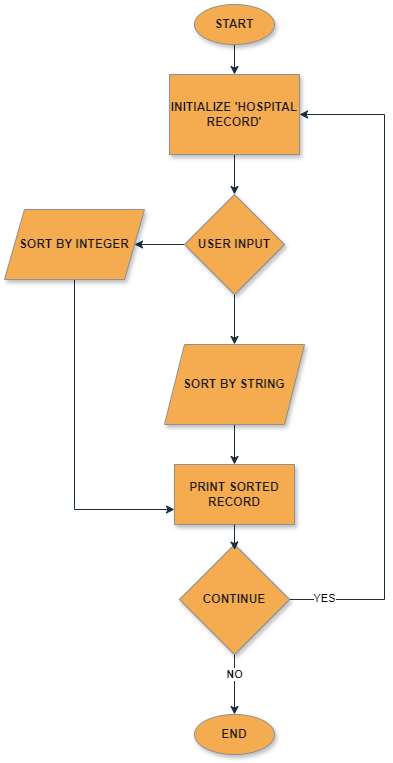
\includegraphics[]{Flow chart/CSE211 Project Hospital Record (radix sort) - flowchart.png}
       \addlinespace
       \caption{Fig: Flowchart }
   \end{center}
   The radix sort methodology involves using counting sort to numerically sort patient records by IDs or ages and to lexicographically sort string attributes. For numerical sorting, the maximum value is calculated to determine sorting iterations per digit, organizing records based on digit values. String sorting involves standardizing string lengths and sorting characters to achieve lexicographical order. The counting sort method categorizes and tallies occurrences of specific digit values or characters, updating the original array with sorted records after processing all digits or characters.
		\end{alertblock}
			
			
		\end{column}
	
		\separatorcolumn
		
		\begin{column}{\colwidth}
			
			\begin{alertblock}{Substitute Use of the Algorithm}{}
            
           Radix sort finds applications beyond sorting hospital records and can be effectively used in various scenarios where keys are represented in a fixed-length format or can be processed digit by digit. One such application is in sorting \textbf{large volumes of numerical data}, particularly in data analysis and scientific computing.
            \addlinespace
            In data analysis tasks, datasets often contain numerical values, such as sensor readings, financial transactions, or scientific measurements. Radix sort can efficiently sort these datasets based on numerical values, providing valuable insights and facilitating further analysis.
            \addlinespace
            \textit{Runtime Complexity:}
            
            \begin{itemize}
                \item Radix sort has a linear time complexity of $O(d*(n+k))$, where d is the maximum number of digits in the numerical values, $n$ is the number of elements to be sorted, and k is the range of the input.
            \end{itemize}
            
            \begin{itemize}
                \item For numerical data with a fixed number of digits or a limited range, radix sort can achieve optimal performance, often outperforming comparison-based sorting algorithms like quick sort or merge sort.
            \end{itemize}


            \textit{Space Complexity:}
            
            \begin{itemize}
                \item Radix sort typically has a space complexity of $O(n+k)$, where n is the number of elements to be sorted and $k$ is the range of the input.
            \end{itemize}
            
            \begin{itemize}
                \item In the context of sorting numerical data, the space complexity remains efficient and scales well with the size of the dataset.
            \end{itemize}
            
            
            In conclusion, radix sort's efficiency and scalability make it a valuable algorithm for sorting numerical data in various applications, including data analysis, scientific computing, and financial analysis. Its linear runtime complexity and space efficiency make it well-suited for handling large volumes of numerical data effectively.
            
            
                        
            			\end{alertblock}
   
   		\begin{alertblock}{Alternative Solution}
			\justifying
    Hospital records can be sorted using quick sort, an adaptable and effective sorting algorithm, based on a variety of criteria, including string and numeric fields. Quick sort can effectively handle a variety of data types and is not limited by specific properties of the data, such as fixed-length keys, as radix sort is. Quick sort is appropriate for situations where performance is crucial because, on average, it is faster than radix sort for larger datasets, with an O(n log n) time complexity. Furthermore, quick sort is an in-place sorting algorithm that uses less memory than radix sort, which might need extra storage in proportion to the range of key values.


             
			\end{alertblock}
   
			\begin{alertblock}{Conclusion}
			\justifying
             Radix sort's linear time complexity makes it faster than comparison-based algorithms like quicksort and merge sort for large datasets. It maintains relative order, making it valuable in real-world applications, and is efficient for sorting large numbers of integers or strings. However, it's not suitable for sorting floating-point numbers, requires significant memory, and isn't efficient for small datasets or those with few unique keys. Despite these drawbacks, radix sort is useful in digital forensics for sorting and analyzing file system metadata, aiding investigators in reconstructing timelines and identifying patterns.


             
			\end{alertblock}
		\end{column}
		
		\separatorcolumn
	\end{columns}
    \end{frame}
\end{document}